\section{Introduction}
\subsection{Problem definition}
\frame
{
	\frametitle{Introduction}
	
	\begin{columns}[t,onlytextwidth]
		\hspace*{-1cm}
		
		\column{.99\textwidth}
		\vspace{-0.5cm}
		\begin{itemize}
			\item Goal: Automated appearance-based place detection 
			\item Place is a specific spatial unit or area  
			\item Place detection is a prior step to
			\begin{itemize}
				\item Place recognition
				\item Topological mapping
				\item Semantic scene understanding
			\end{itemize}
		\end{itemize}
	\end{columns}
}
\frame
{
	\frametitle{Introduction}
	
	\begin{columns}[t,onlytextwidth]
		\hspace*{-1cm}
		
		\column{.99\textwidth}
		\vspace{-0.5cm}
		\begin{itemize}
			\item Appearance-based approach
			\begin{itemize}
				\item Suitable for scene content analysis 
				\item Geometric or odometric data may not be avaiable
			\end{itemize}
			\item Challenges
			\begin{itemize}
				\item Appearance variability
				\item Indiscriminate boundaries
			\end{itemize}
		\end{itemize}
	\end{columns}
}
\subsection{Related work}
\frame
{
	\frametitle{Introduction}
	
	\begin{columns}[t,onlytextwidth]
		\hspace*{-1cm}
		
		\column{.99\textwidth}
		\vspace{-0.5cm}
		\begin{itemize}
			\item Related work
			\begin{itemize}
				\item Partioning of incoming sensory data based on similarity
				\item Clustering
				\item Feature types:
				\begin{itemize}
					\item Global: Histograms, Census Transform, GIST \textcolor{red}{\xmark} ~Sensitive
					\item Local: SIFT, SURF \textcolor{red}{\xmark} ~Low level, Matching
					\item Hybrid: BoW, Bubble Space \textcolor{red}{\xmark} ~Low level
				\end{itemize}
			\item Detecting transition regions (i.e. doors, passages, corridors) \textcolor{red}{\xmark} ~Fails if transitions are not obvious 
				
				
			\end{itemize}
			
		\end{itemize}
	\end{columns}
}
\subsection{Related work}
\frame
{
	\frametitle{Introduction}
	
	\begin{columns}[t,onlytextwidth]
		\hspace*{-1cm}
		
		\column{.99\textwidth}
		\vspace{-0.5cm}
		\begin{itemize}
			\item Proposed approach
			\begin{itemize}
				\item Visual segments
				\item Smooth body or head motion assumption
				\item Spatio-temporal coherence of visual segments
			\end{itemize}
			
			\item Advantages:
			\begin{itemize}
				\item More stable features
				\item Segments Summary Graphs representation
			\end{itemize}
			
		\end{itemize}
	\end{columns}
}
\subsection{General approach}
\frame
{
	\frametitle{General Approach}
	
	\begin{columns}[t,onlytextwidth]
		\hspace*{-1cm}
		
		\column{.99\textwidth}
		\vspace{-0.5cm}
		\begin{figure}[p]
			\centering
			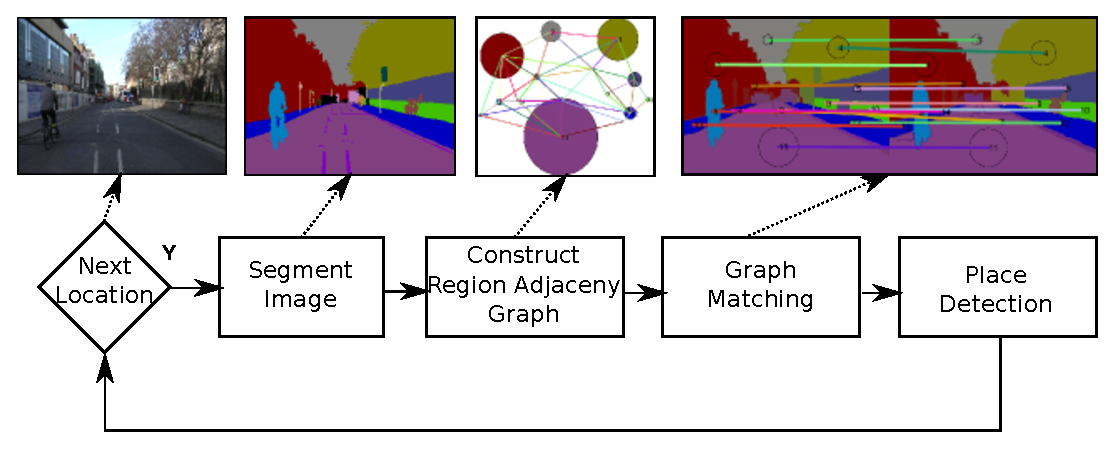
\includegraphics[width = 0.9\textwidth]{img/icsc/diagram_approach}
		\end{figure}
		
	\end{columns}
}